% The Slide Definitions
%document
\documentclass[10pt]{beamer}
%theme
\usetheme{metropolis}
% packages
\usepackage{color}
\usepackage{listings}
\usepackage[ngerman]{babel}
\usepackage[utf8]{inputenc}
\usepackage{multicol}


% color definitions
\definecolor{mygreen}{rgb}{0,0.6,0}
\definecolor{mygray}{rgb}{0.5,0.5,0.5}
\definecolor{mymauve}{rgb}{0.58,0,0.82}

\lstset{
    backgroundcolor=\color{white},
    % choose the background color;
    % you must add \usepackage{color} or \usepackage{xcolor}
    basicstyle=\footnotesize\ttfamily,
    % the size of the fonts that are used for the code
    breakatwhitespace=false,
    % sets if automatic breaks should only happen at whitespace
    breaklines=true,                 % sets automatic line breaking
    captionpos=b,                    % sets the caption-position to bottom
    commentstyle=\color{mygreen},    % comment style
    % deletekeywords={...},
    % if you want to delete keywords from the given language
    extendedchars=true,
    % lets you use non-ASCII characters;
    % for 8-bits encodings only, does not work with UTF-8
    literate={ä}{{\"a}}1 {ü}{{\"u}}1 {ö}{{\"o}}1 {Ä}{{\"A}}1 {Ü}{{\"U}}1 {Ö}{{\"O}}1 {ß}{{\ss{}}}1,
    % escapes umlauts
    frame=single,                    % adds a frame around the code
    keepspaces=true,
    % keeps spaces in text,
    % useful for keeping indentation of code
    % (possibly needs columns=flexible)
    keywordstyle=\color{blue},       % keyword style
    % morekeywords={*,...},
    % if you want to add more keywords to the set
    numbers=left,
    % where to put the line-numbers; possible values are (none, left, right)
    numbersep=5pt,
    % how far the line-numbers are from the code
    numberstyle=\tiny\color{mygray},
    % the style that is used for the line-numbers
    rulecolor=\color{black},
    % if not set, the frame-color may be changed on line-breaks
    % within not-black text (e.g. comments (green here))
    stepnumber=1,
    % the step between two line-numbers.
    % If it's 1, each line will be numbered
    stringstyle=\color{mymauve},     % string literal style
    tabsize=4,                       % sets default tabsize to 4 spaces
    % show the filename of files included with \lstinputlisting;
    % also try caption instead of title
    language = Python,
	showspaces = false,
	showtabs = false,
	showstringspaces = false,
	escapechar = ,
}

\def\ContinueLineNumber{\lstset{firstnumber=last}}
\def\StartLineAt#1{\lstset{firstnumber=#1}}
\let\numberLineAt\StartLineAt



\newcommand{\codeline}[1]{
	\alert{\texttt{#1}}
}


% Author and Course information
% This Document contains the information about this course.

% Authors of the slides
\author{Richard Müller, Tom Felber}

% Name of the Course
\institute{Python-Kurs}

% Fancy Logo 
\titlegraphic{\hfill\includegraphics[height=1.25cm]{../templates/fsr_logo_cropped}}



% Custom Bindings
% \newcommand{\codeline}[1]{
%	\alert{\texttt{#1}}
%}


% Presentation title
\title{Mutation und Klassen}
\date{18. November 2021}

\begin{document}
	
\maketitle

\begin{frame}{Gliederung}
	\setbeamertemplate{section in toc}[sections numbered]
	\tableofcontents
\end{frame}

\section{Wiederholung}
\begin{frame}{Wiederholung}
	\textbf{Beim letzten Mal}
	\begin{itemize}
		\item Tupel
		\lstinputlisting[firstline=2,lastline=2]{resources/04tuples/tuples.py}
		\item Dictionary
		\lstinputlisting[firstline=4,lastline=4]{resources/03bool_fun_dict/dicts.py}
	\end{itemize}		
\end{frame}

\section{Gesamtübersicht}
\begin{frame}{Gesamtübersicht}
	\textbf{Themen der nächsten Stunden}
	\begin{itemize}
		\item \alert{Referenzen Erklärung}
		\item  \alert{Klassen}
		\item Imports
		\item Nützlich funktionen zur Iteration
		\item Lambda
		\item File handeling
		\item Listcomprehension
		\item Unpacking
		\item Dekoratoren
	\end{itemize}
\end{frame}

\section{Referenzen und Mutation}
\begin{frame}{Referenzen}
	Python benutzt ein Konzept namens \alert{"Call by Object-Reference"}. 
	
	Alle Objekte, die in einem Programm auftauchen, liegen im Arbeitsspeicher. Variablen dienen dann dazu, um diesen Objekten einen Namen, eine sogenannte \alert{Referenz} zu geben. 
	
	Variablen sind also nicht ihre Objekte selber, sondern bloß Bezeichner für diese.
\end{frame}

\begin{frame}{Referenzen}
	\lstinputlisting[firstline=1,lastline=2]{resources/05mutation_klassen/reference.py}
	Führt man diesen Code aus, so legt Python den String 'Hallo Welt' irgendwo in den Arbeitsspeicher. 
	
	Die Variable \codeline{hallo} ist nun die Referenz. Greift man auf sie zu, so folgt Python der Referenz in den Speicher und liest dort das eigentliche Objekt aus.
\end{frame}

\begin{frame}{Referenzen}
	Ein Objekt kann auch mehrere Bezeichner haben.
	\lstinputlisting[firstline=4,lastline=5]{resources/05mutation_klassen/reference.py}
	Hier ist \codeline{a} der Name für eine Liste. In Zeile 2 wird nun nicht die Liste kopiert, sondern nur die Referenz darauf. \codeline{b} ist also nur ein weiterer Bezeichner für \textit{dieselbe} Liste.
	
	Dieser Sachverhalt wird deutlich, wenn wir versuchen, \codeline{b} zu verändern:
	\lstinputlisting[firstline=7,lastline=7]{resources/05mutation_klassen/reference.py}
	Python folgt \codeline{b} bis zu der Liste und fügt eine \texttt{2} an. Da \codeline{a} immer noch eine Referenz auf dieselbe Liste hat, wird die Veränderung auch ersichtlich, wenn wir uns \codeline{a} statt \codeline{b} anschauen.
\end{frame}

\begin{frame}{Mutable}
	Das Beispiel aus der letzten Folie funktioniert so, weil Listen veränderlich (mutable) sind. Das heißt, die Liste selbst wird beim appenden verändert, sodass die Änderung bei allen Referenzen sichtbar wird. \alert{Die Referenzen selber ändern sich allerdings nicht.} Dieser Sachverhalt gilt für \textit{alle} veränderlichen Objekte.
\end{frame}

\begin{frame}{Immutable}
	Unveränderliche (immutable) Typen, wie Integer oder Strings, verhalten sich anders.
	\lstinputlisting[firstline=9,lastline=12]{resources/05mutation_klassen/reference.py}
	Hier hat ein Integer zwei Referenzen (\codeline{a} und \codeline{b}). Nutzt man nun \codeline{b}, um auf den Integer etwas drauf zu addieren, so kann Python nicht einfach das bestehende Zahlenobjekt verändern, sondern ist gezwungen, ein neues zu erstellen. Anschließend wird die Referenz von \codeline{b} auf das neue Objekt gesetzt, es wird also die Referenz verändert und nicht das Objekt. Daher sind \codeline{a} und \codeline{b} nun nicht mehr das selbe Objekt.
\end{frame}

\begin{frame}{Listen und Referenzen}
	Listen enthalten keine Objekte, sondern nur Referenzen auf diese. Die Objekte selber liegen irgendwo anders.
	\lstinputlisting[firstline=1,lastline=5]{resources/05mutation_klassen/inner_list.py}
	In diesem Beispiel verändert man die innere Liste unabhängig von der äußeren. Trotzdem wird die Veränderung auch in der großen Liste sichtbar, da man wieder nur mehrere Referenzen auf das selbe Objekt hat.
\end{frame}

\section{Klassen und Objekte}
\begin{frame}{Klassen und Objekte}
	Menschen denken in Objekten, denen Eigenschaften und Funktionen zugeordet werden. \linebreak
	\begin{center}
		 \textbf{Ein Rennwagen ist schnell und die Kuh macht "muh".} \linebreak
	\end{center}
	Deswegen eignet sich dieses Konzept gut, um Code intuitiv zu strukturieren.
\end{frame}
\begin{frame}{bekannte Beispiele}
	Listen: \codeline{liste.append('element')}
	\linebreak
	Dictionaries: \codeline{dictionary.keys()}
	\linebreak
	
	Die \codeline{keys()}-Funktion ist Teil des Dictionary Objekts. Eine Liste z.B. hat keine \codeline{keys()}-Funktion. 
	\linebreak\linebreak
	\codeline{liste.keys()} wird fehlschlagen.	
\end{frame}

\begin{frame}
	Mit dem Punkt \codeline{.} kann auf die Funktionen des Objekts und Attribute zugegriffen werden.
	\lstinputlisting[firstline=13,lastline=13]{resources/05mutation_klassen/einleitung_klassen.py}
	Mit den Klammern wird angezeigt, dass man eine Funktion des Objekts ausführen will.
	\lstinputlisting[firstline=14,lastline=14]{resources/05mutation_klassen/einleitung_klassen.py}
	\begin{center}
		\Large Funktion eines Objekts $\,\to\,$ \alert{Methode}
	\end{center}
\end{frame}
\begin{frame}{Klassen / Objekte selbst definieren}
	Um ein Objekt zu erhalten, muss zunächst eine Klasse definiert werden. Anschließend muss diese Klasse ausgeführt (instanziiert) werden. Die \codeline{\_\_init\_\_} Funktion wird jedesmal aufgerufen, wenn eine neue Instanz der Klasse erzeugt wird (Konstruktor).
	\lstinputlisting[firstline=0,lastline=5]{resources/05mutation_klassen/einleitung_klassen.py}
	\lstinputlisting[firstline=13,lastline=13]{resources/05mutation_klassen/einleitung_klassen.py}
\end{frame}
\begin{frame}{self}
	In jeder Methode einer Klasse wird \codeline{self} als Eingabe mitgegeben. \codeline{self} repräsentiert eine Referenz zu dem jeweiligen Objekt, dass die Methode aufgerufen hat.\linebreak
	In der \codeline{\_\_init\_\_} Methode kann \codeline{self} benutzt werden, um die Attribute jeder Instanz der Klasse zu setzen. (Zeile 3)
	\lstinputlisting[firstline=0,lastline=5]{resources/05mutation_klassen/einleitung_klassen.py}
	\lstinputlisting[firstline=13,lastline=13]{resources/05mutation_klassen/einleitung_klassen.py}
\end{frame}
\begin{frame}{Methoden}
	Methoden können nach dem gleichen Schema angelegt werden, wie Funktionen, mit zwei Unterschieden.
	\begin{itemize}
		\item methoden enthalten mindestens \codeline{self} als Eingabe-Argument
		\lstinputlisting[firstline=7,lastline=7]{resources/05mutation_klassen/einleitung_klassen.py}
		\item methoden werden unter Klassen definiert
		\lstinputlisting[firstline=6,lastline=7]{resources/05mutation_klassen/einleitung_klassen.py}
	
	\end{itemize}
\end{frame}
\begin{frame}{Magische Methoden}
	Es gibt einige Methodennamen, die in Klassen reserviert sind. Alle starten und enden mit doppeltem Unterstrich. Diese Methoden heißen auch "magic methods", weil sie spezifische Dinge, scheinbar magisch, automatisch passieren lassen:
	 \begin{center}
	 	\codeline{\_\_*f\_name*\_\_} \linebreak\linebreak
	 	\pause
	 	\begin{tabular}{m{2.5cm} | m{6cm}}
	 		Methodenname & Zweck \\ \hline\hline
	 		\codeline{\_\_init\_\_} & Konstruktor: wird bei Objekt() aufgerufen \\ \hline
	 		\codeline{\_\_str\_\_} & bestimmt Rückgabewert von str(Objekt) \\
	 		\hline
	 		\codeline{\_\_add\_\_} & bestimmt Rückgamewert Objekt + Objekt \\
	 	\end{tabular}
	 \end{center} 
\end{frame}


\section*{Beispiel}
\begin{frame}
	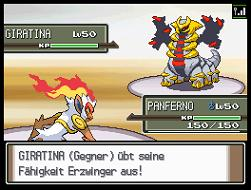
\includegraphics[width=\linewidth]{resources/05mutation_klassen/pokemon_ballte.jpeg}
\end{frame}
\begin{frame}{Beispiel}
	\textbf{Problemmodellierung:}
	Pokemon
	\begin{itemize}
		\item Eigenschaften
		\begin{itemize}
			\item Name
			\item maximale HP (Health Points)
			\item aktuelle HP
			\item Angriffs Kraft
		\end{itemize}
		\item Aktionen / Funktionen
		\begin{itemize}
			\item angegriffen werden
			\item anderes Pokemon angreifen
			\item geheilt werden
		\end{itemize}
	\end{itemize}
	zu beachten:
	\begin{itemize}
		\item HP sollen nicht unter 0 sinken
		\item Pokemon mit 0 HP können nicht angreifen
	\end{itemize}

\end{frame}
\end{document}
